\par Le membre du groupe responsable de cette partie était Antoine Vallée.

\par Dans un Shoot Them All, l'intelligence artificielle n'est pas vraiment présente dans la plupart des phases du jeu: Les ennemis de base n'effectuent que de simple actions qui se révèlent être toujours les même. Toutefois, il nous paraissait important de travailler sur cet aspect des jeux vidéos, qui nous parait primordiale.
\par C'est pourquoi nous avons très vite décidé que des boss seraient présents dans le jeu, et qu'ils traduiraient concrètement notre travail sur l'intelligence artificielle. Nous nous étions fixé un objectif de 5 boss, et nous y sommes arrivé, sans trop de mal d'ailleurs. Seul un membre du projet aura eu à se concentrer sur cette tâche.
\par Pour développer nos boss, nous nous sommes inspirés de jeux récents ayant faits leur succès dans l'intelligence artificielle, en nous basant sur un système largement répandu, mais aussi très efficace, de phases. En effet, chaque combat contre un boss est divisé en plusieurs phases, qui se déclenchent en fonction de la vie du boss ou du temps écoulé. Ce système de phase est primordiale car il apporte une dynamisme au combat qu'aucun autre système ne saurait apporter. Il permet de ne pas geler le boss à une seule stratégie, qu'il appliquera tout le long du combat, mais de lui donner la possibilité d'appliquer plus de 3 stratégies différentes en fonction des situations.
\par Avec ces changements de stratégies en plein combat, le joueur se retrouve à devoir constamment changer de tactique pour ne pas mourir et pour éliminer le boss. Graphiquement cela demande un travail colossal en plus (nombreux missiles par boss, météorites etc..), mais ça en vaut la peine.
\par Ainsi, nous avons développé ces boss au fur et à mesure de l'année, nous en avons présenté un à la première soutenance, qui fut le plus long à développer puisqu'il fallait créer toute la structure même des boss, puis nous en avons présenté trois en troisième soutenance, pour finir avec un total de cinq sur la version finale du projet.

	\par 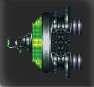
\includegraphics[width=13cm]{images/boss1.jpg}   Nom: Spaceship X-42
               Tactique: En phase 1, le boss va tirer des salves de missiles tout en se déplaçant de haut en bas. Une fois entré en pahse 2, il va se déplacer beaucoup plus vite et le joueur devra vite lui faire perdre de la vie. La phase 3 est elle, bien plus intéressante: Le boss devient invincible, entouré d'un bouclier bleu. Il tire sans s'arrêter, puis perd son bouclier quelques secondes. C'est à ce moment là que le joueur doit le toucher, tout en évitant ses missiles dévastateurs.
			   
\par 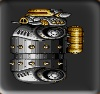
\includegraphics[width=13cm]{images/boss2.jpg}   Nom: Metal'Krisboul
				Tactique: En phase 1, le boss va seulement se déplacer de haut en bas sans tirer. Toutefois en phase 2 une pluie de météores va s'abbattre sur le joueur, qui va devoir les éviter tout en continuant de tirer sur le boss. Passée cette pluie, le boss va se mettre à tirer des salves de trois missiles, dont deux en diagonales qui feront perdre énormément de vie au joueur. Bonne chance !
				
\par 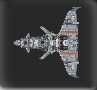
\includegraphics[width=13cm]{images/boss3.jpg} Nom: Tie supressor
				Tactique: En première phase, le boss va tirer des salves de missiles. Puis, une fois en danger, il va se replier et appeler en renfort de nombreux ennemis. Le joueur devra les détruire, et affaiblir le boss une fois réapparu. Si il ne le tue pas assez vite, d'autres renforts vont arriver, et il se retrouvera vite submergé.
				
\par 
\includegraphics[width=13cm]{images/boss45.jpg} Nom: The All-Seeing Eye
				Tactique: Ce boss peut paraitre anodin à première vue: Un simple oeil. Mais détrompez vous, malgré une phase 1 relativement simple (un simple tir de missile), la suite va être très corsée. En effet, le boss va se téléporter dans tout l'écran, créant autour de lui un énorme cercle que le joueur devra absolument éviter. Ce dernier n'aura qu'une seconde pour réagir et se déplacer avant l'apparition du cercle, tout en ayant sa vitesse extrêmement réduite. Il devra aussi faire preuve de rapidité et tirer sur le boss une fois 4 téléportations effectuées: C'est à ce moment là qu'il ne sera plus intouchable.
				
			    Nom: NathalisBoulax
				Tactique: Surprise.
				
\par Et une image pour la route !
\par 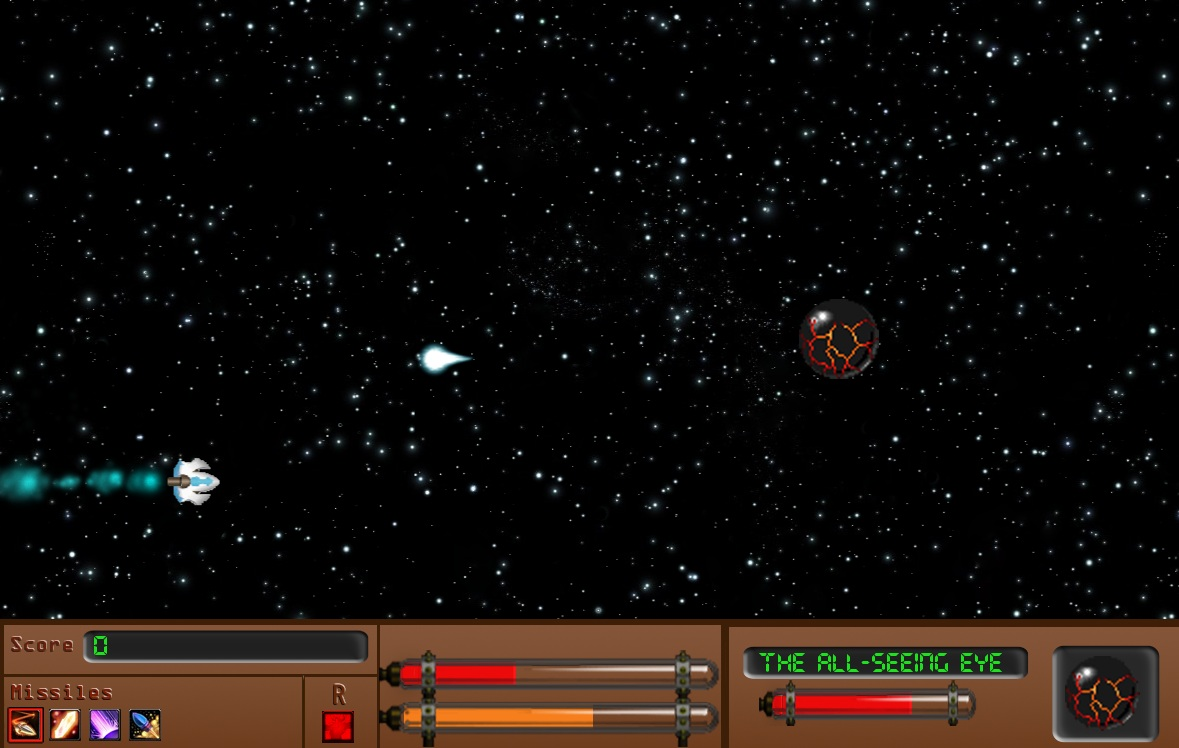
\includegraphics[width=13cm]{images/boss42.jpg}
